% \paragraph{Summary}

We have developed a novel Bayesian nonparametric model for spike sorting called \smug.  Our model and inference procedure incorporate certain features that previous approaches---be they nonparametric or not---lacked.  Most importantly, we developed a variational Bayesian online inference scheme, that enabled faster than real-time posterior inference.  Such computational efficiency is crucial for sequential experimental design \cite{}.  Although we only provided our algorithm with streaming data, \smug\ outperformed all competitor \emph{batch} algorithms (that is, algorithms that consume all the data at once). Our improved sensitivity and specificity seem to arise from multiple sources including (i) improved detection, (ii) correlated noise, (iii) capturing overlapping spikes, (iv) tracking waveform dynamics, and (v) utilizing multiple channels.  While others have developed closely related Bayesian models for clustering \cite{WoodBla2008,wood2009}, deconvolution based techniques \cite{Pillow2013}, time-varying waveforms \cite{calabrese2011kalman},  \emph{or} online methods \cite{OSORT, Franke2010}, we are the first to our knowledge to incorporate \emph{all} of those features.

An interesting implication of our work is that it seems that our errors result from problems of the dictionary.  Fig.\ \ref{fig:ICold} shows the true positives, missed positives, and false positives in the space of the first two PCs (see Supplementary Fig.\ \ref{pairs}). Although we are clustering in a higher dimensional subspace (5 PCs) 

% \vspace{-10pt}
\paragraph{Limitations of Dictionary-Based Techniques} \label{sub:template}
\vspace{-5pt}


\begin{center}
\begin{figure}[h!]
\begin{subfigure}[b]{.33\textwidth}
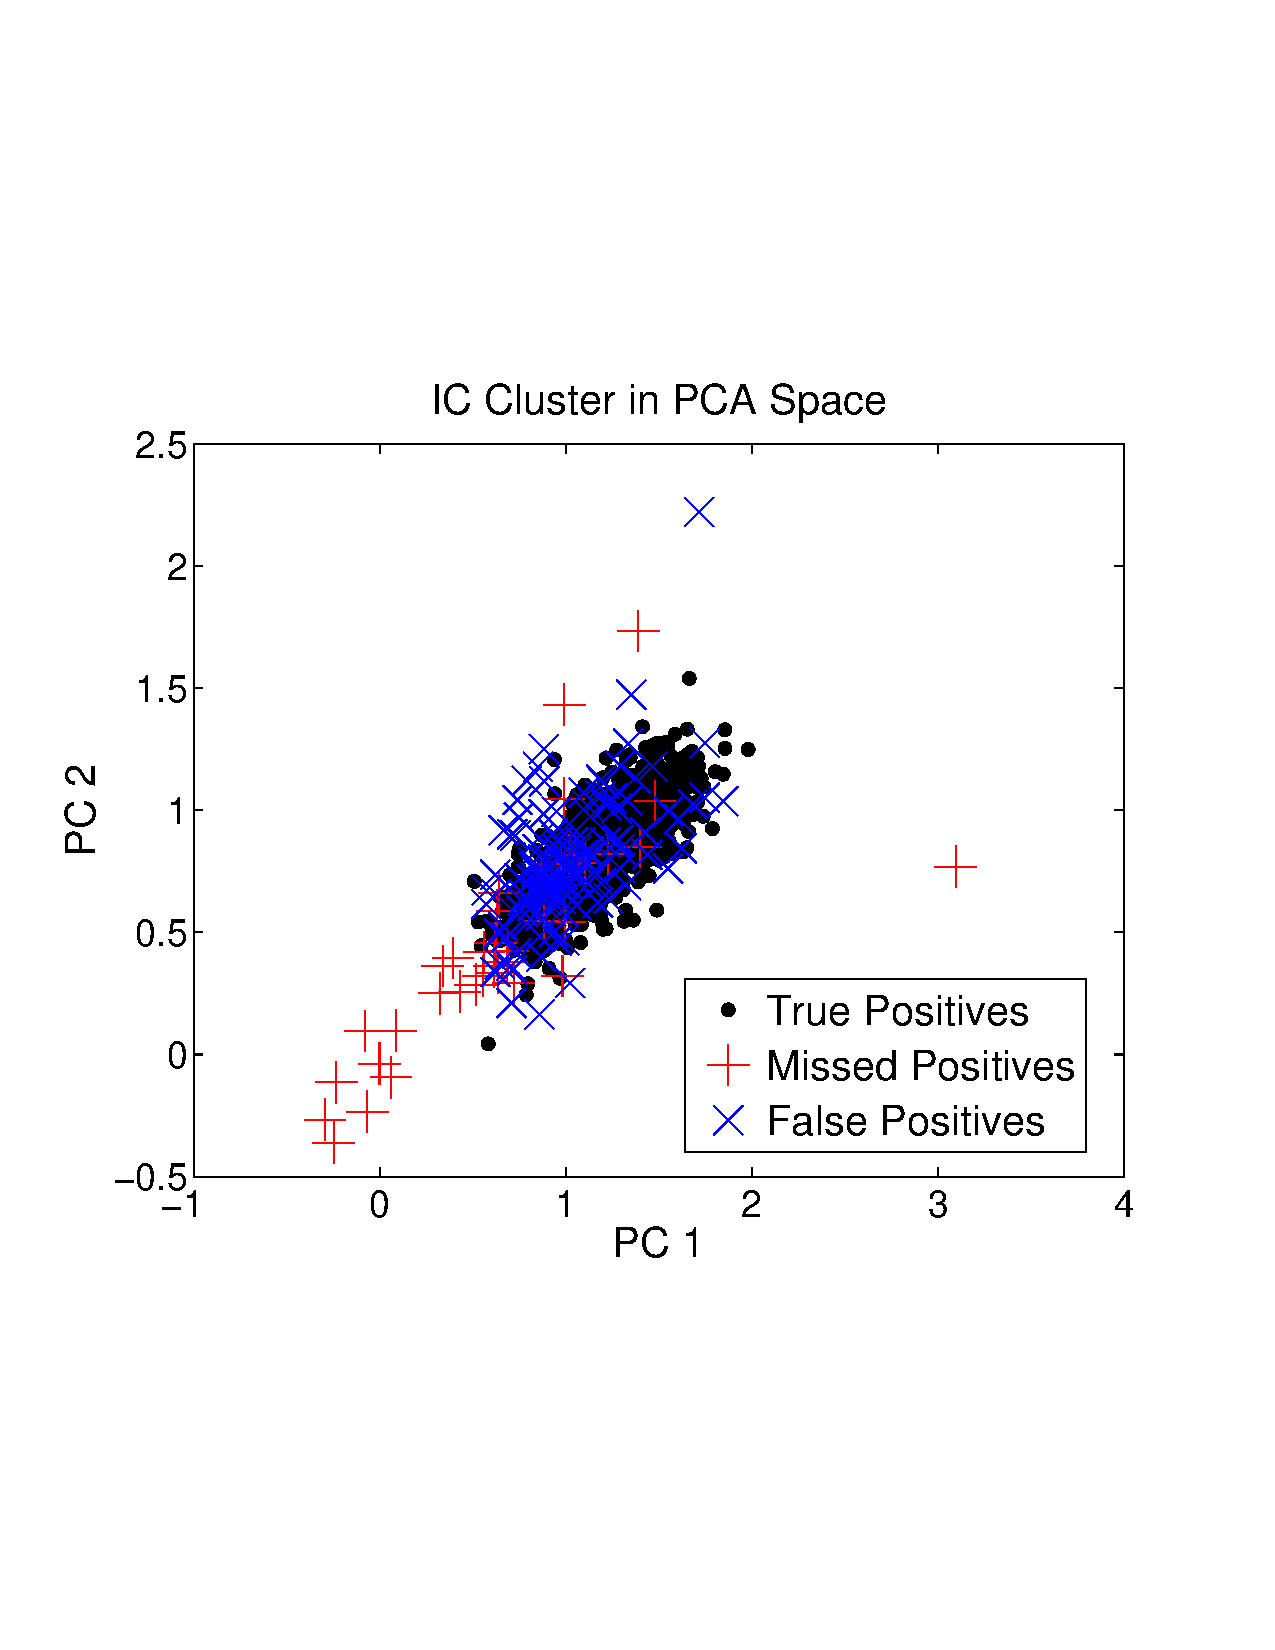
\includegraphics[width=\textwidth]{../figs/new/ICclusteroldpca.pdf}
\caption{}
\label{fig:ICold}
\end{subfigure}
\begin{subfigure}[b]{.33\textwidth}
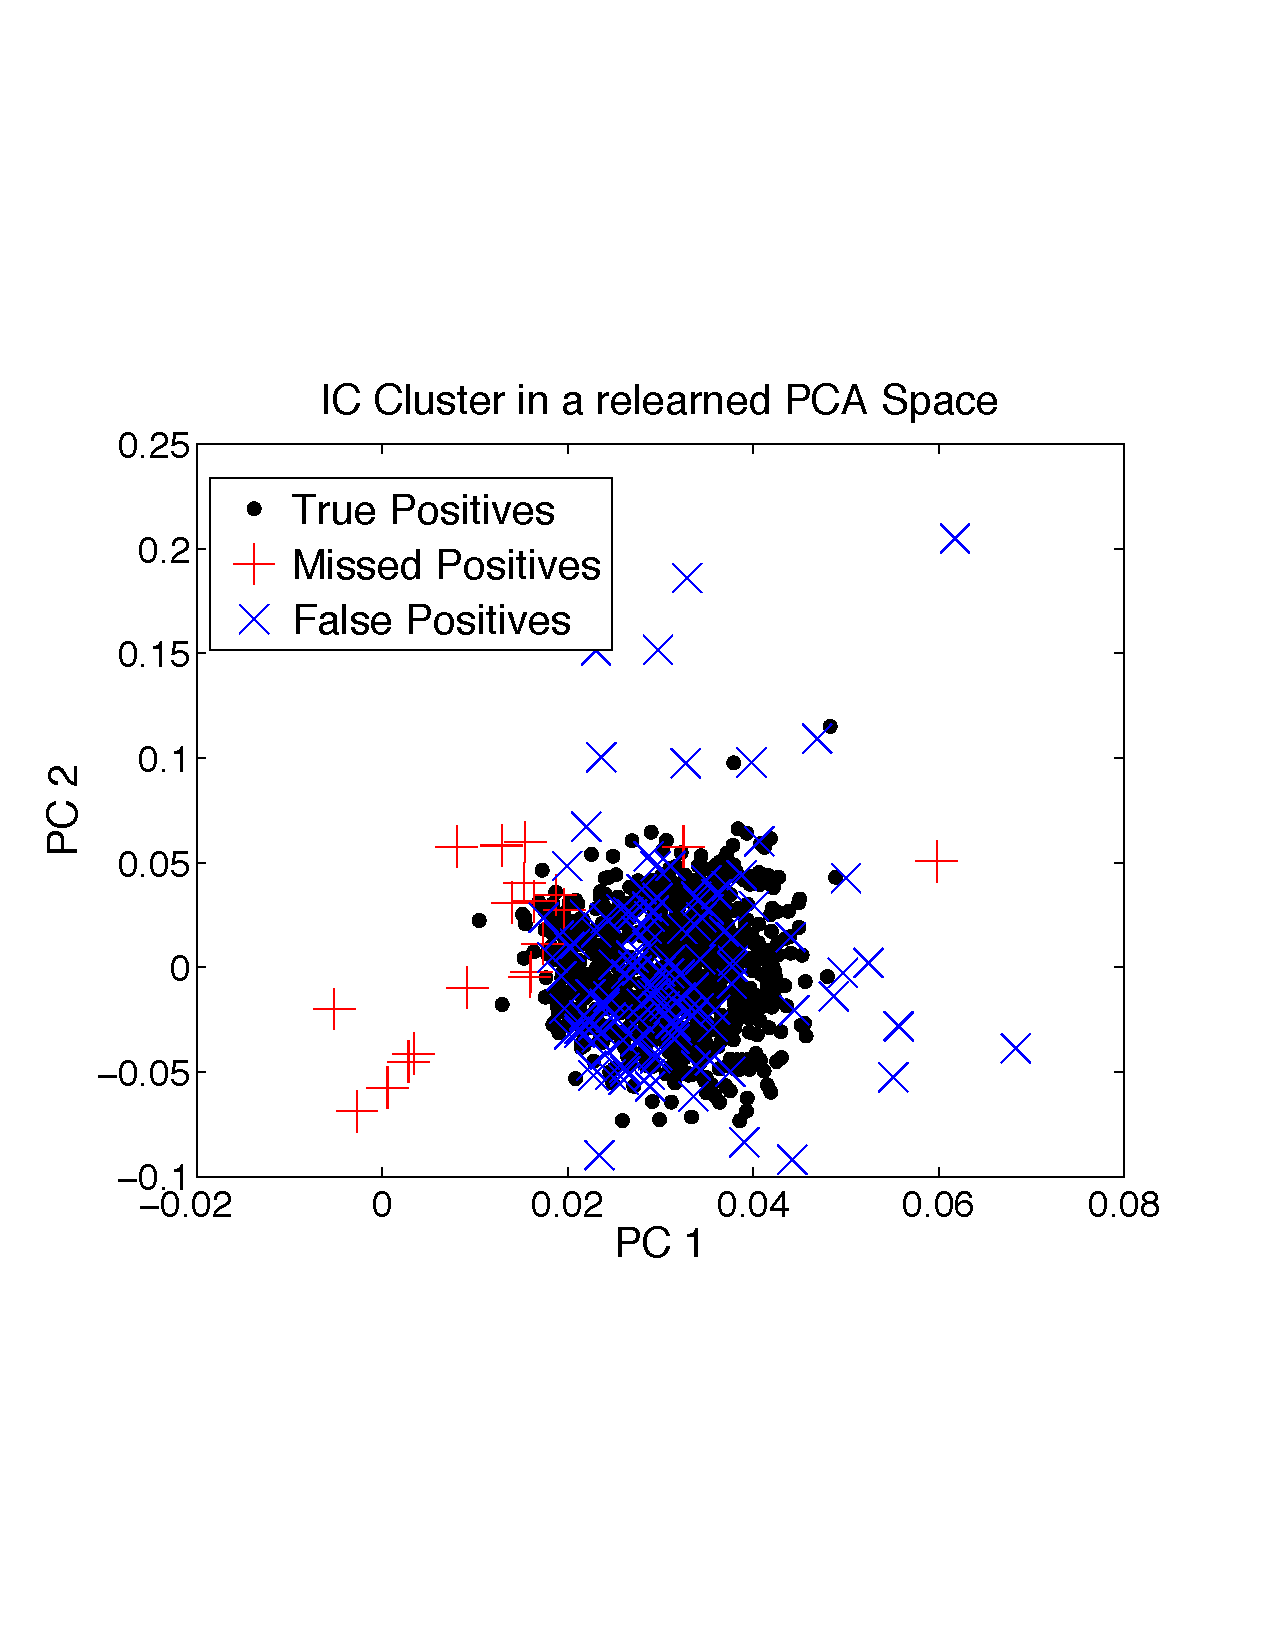
\includegraphics[width=\textwidth]{../figs/new/ICclusternewpca.pdf}
\caption{}
\label{fig:ICnew}
\end{subfigure}
\begin{subfigure}[b]{.33\textwidth}
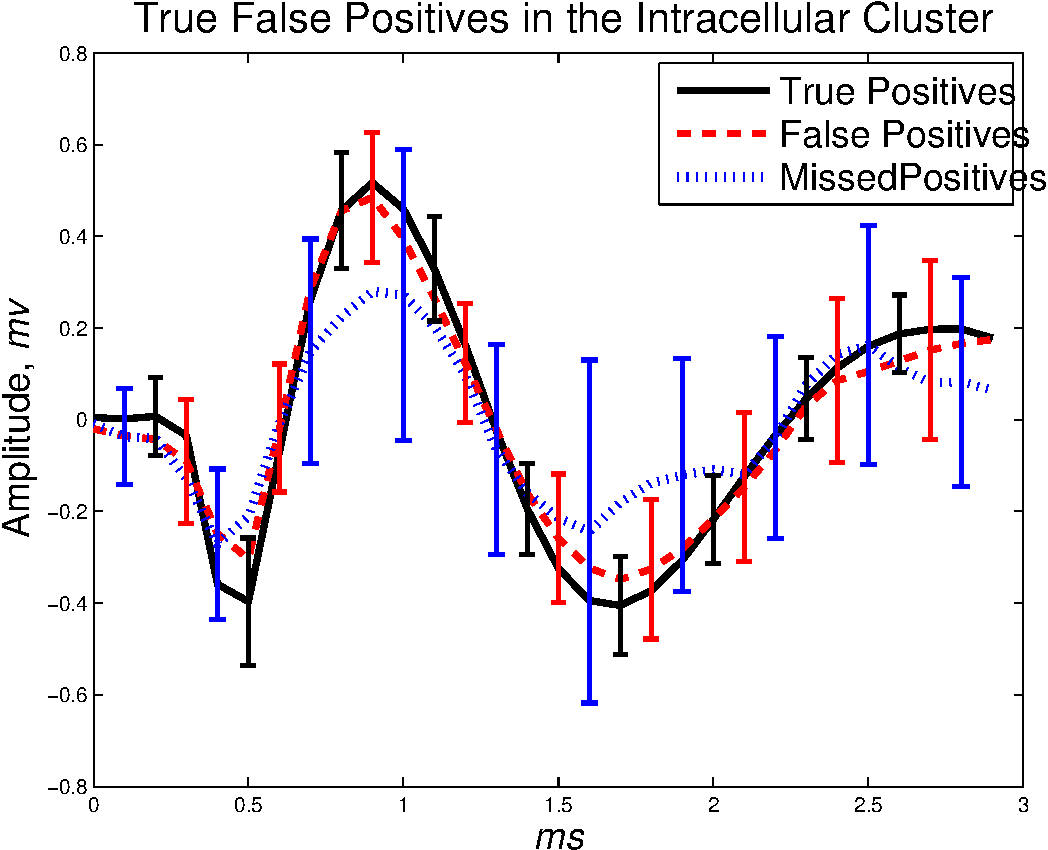
\includegraphics[width=\textwidth]{../figs/IntracellularTrueFalsePositivesv2}
\caption{}
\label{truewaveforms}
\end{subfigure}
\caption{Template matching.
(c) Errorbar plots of the true positives and the false positives in the IC cluster.  While the false positives have slightly more variability, the mean shape for the false positives and the true positives is nearly identical.  The true misses have a significantly lower amplitude as well as high variability. 
} \label{fig:IC-PCA}
\end{figure}
\end{center}




in discussion:

embarrassingly parallel per 4

ignore time steps that aren't useful

let $\lambda_i$ vary as a function of: (i) spike histories, (ii) stimulus, (iii) possibly baseline drift?


\clearpage
\section{comments}

{\color{red} perhaps add comments about time-evolution and the false positives we avoid by using multi-channel analysis}

\jovo{add grids to all panels of all figs by default, remove if it looks shitty.}

\jovo{@dec - for fig 1 keep colors/symbols the same in the two panel, if possible.  maybe use a scheme where color indicates algorithm and shape indicates \# of components.  also, be consistent about "IC" cluster vs. "Intracellular" Cluster. and normalize, renaming axes XY Rate instead of only XY. (b) title should be ``ROC Curve Comparisons''}  


